\subsection{Image Processing}

In order to localize the robot 3D, the position of the location of the robot and of the $N$ reference points need to be determined. The implemented procedure is based on bright colored, circular reference points and is semi-automatic.

While the precise location of the centers of the reference points is calculated automatically, the user defines the regions of interest and the relative position of the reference points by clicking in order on these points. (see Figure). Examining the picture's HSV representation (Figures  and ), one can see that a combination of the H and S values gives can deliver a good criteria for the extraction of the bright colored points. Hence, the colors are extracted in two steps: first a rough filter is applied to the image, which is then refined by only keeping the main part of the colors left. (FORMULAS) (Figure, green lines mark the contours of the extracted color regions).

-> algorithms:
color extraction
contours
circles



%\begin{lstlisting}[caption=Listing]
%\end{lstlisting}

%\begin{figure}[H]
%	\centering
%	\begin{subfigure}[b]{0.49\linewidth}
%		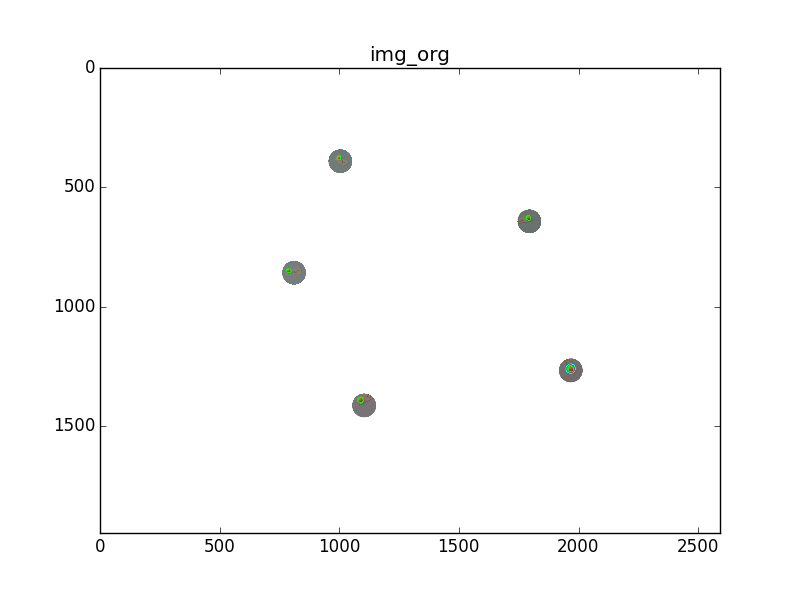
\includegraphics[width=\linewidth]{../files/img_org139.png}
%		\caption{Regions of interest chosen by user and extracted colors}
%		\label{feat_step0}
%	\end{subfigure}
%	\begin{subfigure}[b]{0.49\linewidth}
%		\includegraphics[width=\linewidth]{../files/img_h139.png}
%		\caption{\textit{Hue} representation of original image}
%		\label{feat_step1}
%	\end{subfigure}
%	\begin{subfigure}[b]{0.49\linewidth}
%		\includegraphics[width=\linewidth]{../files/img_s139.png}
%		\caption{\textit{Saturation} representation of original image}
%		\label{feat_step2}
%	\end{subfigure}
%	\begin{subfigure}[b]{0.49\linewidth}
%		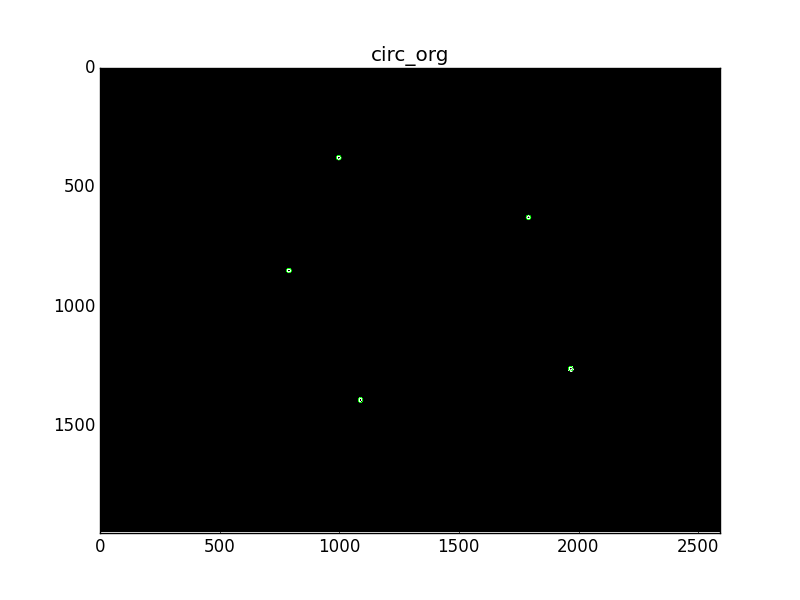
\includegraphics[width=\linewidth]{../files/circ_org139.png}
%		\caption{Regions of interest chosen by user and extracted colors}
%		\label{feat_step3}
%	\end{subfigure}
%	
%	
%	\begin{subfigure}[b]{0.49\linewidth}
%		\includegraphics[width=\linewidth]{../files/zdot_RefTrackNL.png}
%	\end{subfigure}
%	\begin{subfigure}[b]{0.49\linewidth}
%		\includegraphics[width=\linewidth]{../files/speeds_RefTrackNL.png}
%	\end{subfigure}
%	\begin{subfigure}[b]{0.49\linewidth}
%		\includegraphics[width=\linewidth]{../files/xyz_RefTrackNL.png}
%	\end{subfigure}
%	\caption{Procedure for feature extraction} 
%	\label{features}
%\end{figure}
